\graphicspath{{Images/}}

\section{NIST's PQC Standardization Competition} \label{industry}
In 2009, NIST published a PQC survey, but it wasn't until 2012 that they announced the PQC competition. Spurred on by the announcement made by the NSA that the US government systems would be pursuing quantum-safe solutions, NIST published a report on PQC (\textbf{\gls{nistir}} 8105), devised a timeline, a series of submissions criteria, as well criteria by which to judge and test submissions. The rules and guidelines of the competition were presented at the PQCrypto Conference in 2016 in Japan with the caveat that such standards and rules may shift and change with input from the community. No stranger to competitions, NIST has successfully used similar competitions to standardize 
    the Diffie-Hellman and Elliptic Curve Diffie-Hellman protocol (\textbf{\gls{ecdh}})(which resulted in \textbf{\gls{sp}} 800-56A),
    the RSA encryption scheme (SP 800-56B, \textbf{\gls{fips}} 186),
    DSA and Elliptic Curve DSA (\textbf{\gls{ecdsa}})(FIPS 186), 
    and more.
All of these past standards however were liable to be vulnerable to attack should a CRQC become available, and despite the familiarity of the process of standardizing new algorithms or updating standards for algorithms already in existence, the task of finding post-quantum algorithms to standardize and recommend was a much larger task that before because 
    (1) post-quantum cryptography was going to be more complicated than the cryptography required for past competitions, 
    (2) there would be no ``silver bullet" because all algorithms would have benefits and weaknesses (NIST stated in addition they'd ideally like to choose more than one ``winner"), 
    (3) the algorithms chosen must be able to work on a wide variety of systems, and 
    (4) they must be able to be run and be tested on classical systems while being quantum-safe. 

\begin{figure}[h] 
    \centering
    \ffigbox[\FBwidth]
        {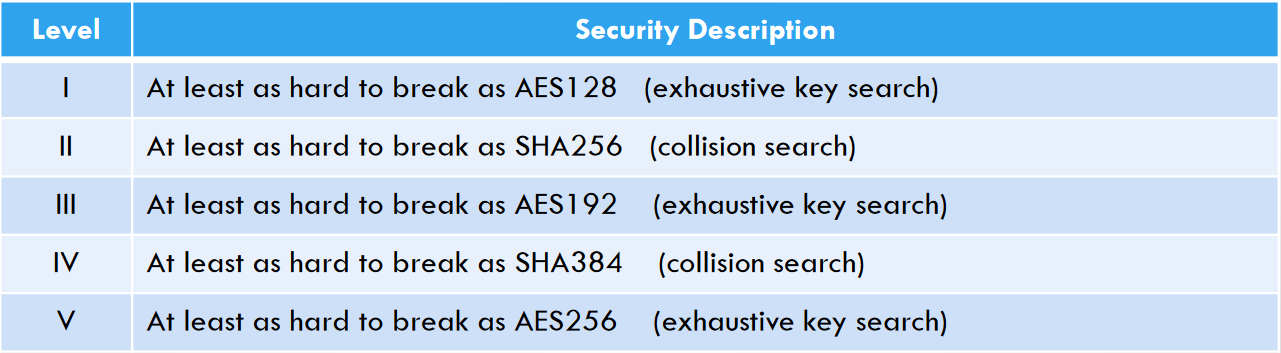
\includegraphics[width=0.75\textwidth]{security_lvls.png}}
        {
            \captionsetup{justification=centering}
            \caption{NIST's levels of security on which algorithms would be graded}
            \label{fig:sec_levels}
        }
\end{figure}

Included in this announcement, they stated that they would be looking for digital signature, encryption, and key exchange algorithms (\textbf{\glspl{kem}}) (while not being part of the official competition, they later announced that they would be looking for proposals for stateful hash-based signature algorithms as well). They expressed the desire for algorithms that would cover these three bases while being based on a variety of different types of quantum algorithms. In their solicitation for proposals and papers, they stated that submissions should be publicly disclosed and freely available, having signed statements with patent information disclosed, having ``theoretical and empirical evidence providing justification for security claims", and including ``concrete...parameters for meeting target security levels" (see Figure \ref{fig:sec_levels}) \cite{moody_ship_sailed}.

In addition to security, they stated that algorithms would be judged on performance. Algorithm capable of additional features would be considered even better. Examples of additional features that NIST was looking for included:
\begin{itemize}
    \item``drop-in replacements - compatibility with existing protocols and networks,
    \item perfect \textbf{\gls{forwardsecrecy}},
    \item resistance to \textbf{\glspl{sidechannelattack}},
    \item simplicity and flexibility,
    \item misuse resistance" \cite{moody_fourth},
    \item and any other additional features similar to those already stated
\end{itemize}

In a presentation given by Dustin Moody (NIST Fed) at the AsiaCrypt conference in 2017, NIST described their role as ``managing a process of achieving community consensus in a transparent and timely manner" \cite{moody_ship_sailed}.

\subsection{Off to the Races}
In the initial set of submissions, NIST received 82 papers with 69 papers meeting the minimal submissions criteria, being considered "complete and proper" \cite{moody_lets_2018}. Round over round and year after year, progress marked by continued presentations, workshops, and conferences whittled the number of algorithms in the running down quickly. Algorithms were eliminated for a variety of reasons such as being broken, significantly attacked, NIST lacking full confidence in their security, or the algorithms being deemed too inefficient. There were small alterations to submissions criteria and judging criteria made to incorporate feedback from the community and introduce a bit more flexibility. Some submissions were added in later rounds while other similar ones were merged, and some submissions were given suggestions to make improvements into order to move forward in the competition. As is illustrated in Figures \ref{fig:algossorted} and \ref{fig:algosbreakdown}, there were a variety of algorithms for encryption and key exchange as well as signatures which were split into several categories based on the type of quantum algorithm they utilized. By the end of the third round in 2022, four algorithms had been chosen for standardization: one lattice-based encryption/key exchange protocol, two lattice-based\footnote{refers to the type of quantum algorithm used, namely, it refers the quantum physics property or scheme that allows an algorithm built on it to be secure} \footnote{types of quantum algorithms include: 
(structured and unstructured) lattice-based (module learning with errors, module learning with rounding), isogeny based, code-based (Goppa, short Hamming, low rank), symmetric-based, hash-based, multivariate-based schemes, and more.} digital signature schemes, and one hash-based digital signature scheme. A quick summary of each is given as follows:

\begin{figure}
    \centering
    \ffigbox[\FBwidth]
        {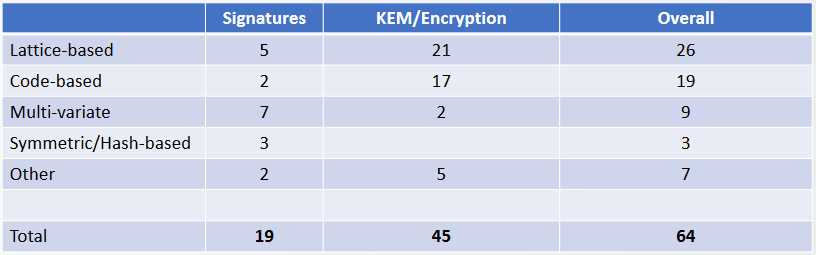
\includegraphics[width=0.65\textwidth]{algosbreakdown.png}}
        {
            \captionsetup{justification=centering}
            \caption{The breakdown of algorithms submitted in the first round. The majority were lattice-based encryption/key exchange protocols \cite{moody_lets_2018}}
            \label{fig:algosbreakdown}
        }
\end{figure}
\begin{figure}
    \centering
    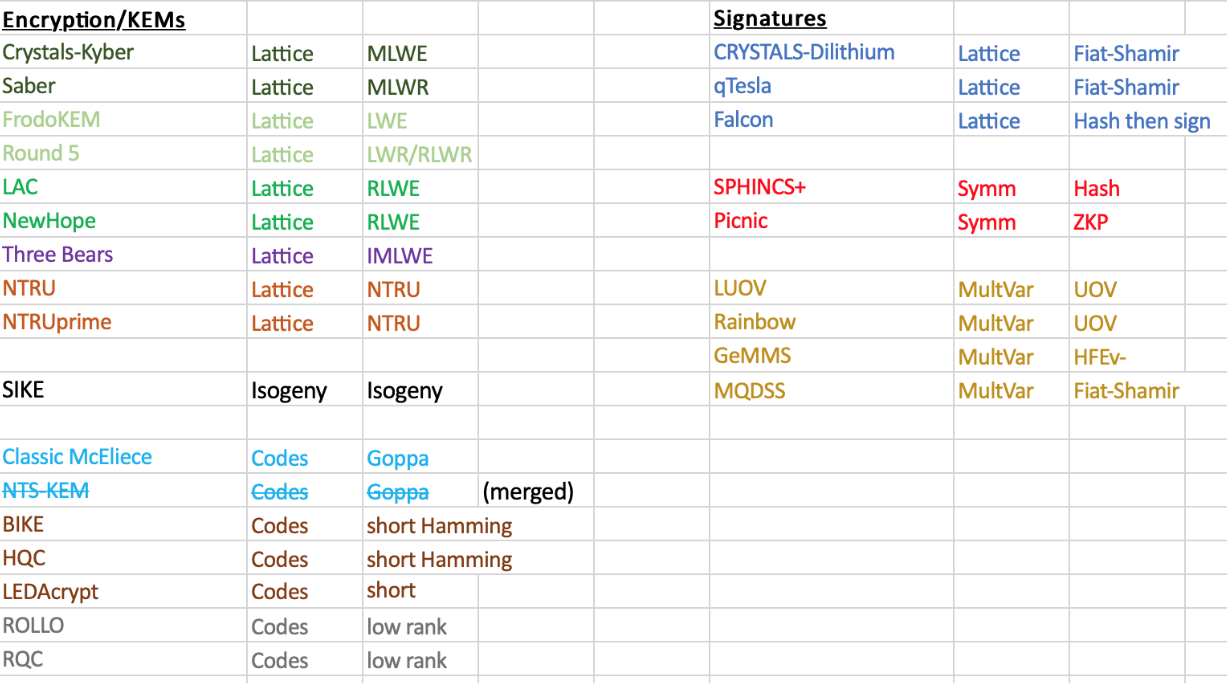
\includegraphics[width=0.75\linewidth]{Images/algos_sorted.png}
    \caption{The list of second round candidates sorted by algorithm type \cite{moody_round2}}
    \label{fig:algossorted}
\end{figure}

\subsection{CRYSTALS-Kyber}
The only public-key encryption/key exchange protocol chosen for standardization at the end of the third round was CRYSTALS-Kyber which was based on structured lattices and the module learning with errors problem. Designed to have IND-CCA2\footnote{indistinguishability under adaptive chose ciphertext attack} 
base level security when used for key exchange and IND-CPA\footnote{indistinguishability under chosen plaintext attack} 
base level security when used for encryption, it was chosen for its ``strong security and performance" \cite{moody_fourth}. NIST stated they would standardize sub-schemes Kyber-768 (providing level 3 security, see Figure \ref{fig:sec_levels}) and Kyber-1024 (providing level 4 security), and they were considering standardizing Kyber-512 as well (at the time of the fourth round they stated that this was just barely meeting level 1 security but it could be advantageous to standardize due to the current cost, stating it would be offered as a smaller alternative). This culminated in Draft FIPS 203 released August 24, 2023 which closed its public comment period on November 22, 2023.

\subsection{CRYSTALS-Dilithium}
One of the two structured lattice-based digital signature schemes chosen for standardization was from the same team as CRYSTALS-Kyber. CRYSTALS-Dilithium used a ``Schnorr-like" \cite{dilithium} lattice-based scheme, supported by the module learning with errors problem. It was chosen for its "strong security and performance", and NIST stated that they planned to standardize the parameter sets that corresponded with ``security categories 2, 3, and 5" \cite{moody_fourth}. This culminated in Draft FIPS 204 released August 24, 2023 which also closed its public comment period on November 22, 2023. 

\subsection{Falcon}
Falcon is the second of the two structured lattice-based digital signature schemes and third of the overall schemes chosen for standardization. It was chosen for standardization as a possible alternative for applications where the CRYSTALS-Dilithium signature was too large. When the team behind Falcon were tasked with presenting their scheme they laid out how their scheme is different, its strengths, its weakness, as well as some ideal applications. Falcon is the only scheme that uses floating point arithmetic and as such must be run on systems with floating point units (\textbf{\gls{fpu}}). This could pose a limitation on its adoption in the case of devices without FPUs, with FPU emulators, or variable-time FPUs. Where systems use emulators or variable-time FPUs, the performance of Falcon may be slower or less reliable, and for companies trying to keep the scheme they use secret, Falcon would not be the best choice because of its unique implementation. The team described vehicle-to-vehicle communications, TLS certificates, systems that don't have a lot of resources for verification, and DNSSEC\footnote{Domain Name System Security Extensions} as ideal applications. NIST announced that they would write the draft standard document for Falcon after completing those for Kyber, Dilithium, and SPHINCS+ which means that despite not having been published yet, such a draft document for which a public comments period will open is due any day now. 

\subsection{SPHINCS+}
SPHINCS+ is the final scheme chosen for standardization thus far, and it is the only hash-based digital signature scheme chosen for standardization. Chosen for its ``solid security", it was originally listed as an alternate when the finalists were announced during the third round; however, the premise which its security is based has existed long enough to have made SPHINCS+ a safe bet. As such, this resulted in Draft FIPS 205 which closed its period for public comments November 22, 2023.

\subsection{The Fourth Round...}
As it currently stands, the PQC Standardization Competition is technically in its fourth round. As mentioned before three draft FIPS documents have been released, and we are awaiting a fourth for Falcon. NIST announced additional public key encryption/key exchange protocols BIKE, Classic McEliece, HQC, and SIKE will be candidates further considered for standardize. They have also released a call for proposals for digital signature algorithms with short signatures and fast verification \cite{announcingfourth}. 

\subsection{... Moving Forward}
The fifth PQC standardization conference is scheduled to be held April 10-12, 2024. On their website they state the purpose will be to ``discuss various aspects of the algorithms (both those selected and those being evaluated) and to obtain valuable feedback for informing decisions on standardization" \cite{announcingfifth} where representative from all teams creating algorithms under consideration will present. When the competition was initially announced, NIST stated that they would like to release standard by 2023. Halfway through the competition they received recommendation that they take their time to ensure a thoughtful and thorough evaluation process. When this decision was made, they amended their statement to say that standards would be available sometime in 2024. The process of not only finding solutions but making sure that the solution found are diverse and robust is an ongoing process which NIST is taking very serious. Coordinating a process in which scientists, mathematicians, physicists, as well as many other types of researchers from all over the world are participating in is a large task to take on, but it has been redeeming to see the ways in which people have come together to create solutions. The process of post-quantum standardization is likely to be an ongoing task that will not end very soon and may not end necessarily when quantum computers arrive. It is much more likely that the coming of a CQRC will create as much if not more excitement, presenting new challenge, we have seen from the discussion of the possibility of one which prompted the PQC competition. It is unclear where this timeline will end, but there have been many promising development to have come out of it. 